
\documentclass[master]{thesis-uestc}

\title{时域积分方程时间步进算法及其快速算法}
\author{王稳}
\advisor{赖生建\chinesespace 副教授}
\school{物理电子学院}
\major{无线电物理}
\studentid{201421040223}

% write all usepackage here
% \usepackage{algorithm2e}

\begin{document}

\makecover

% this is a thesis template with mutiple files: the chapters/ and the misc/ contain related files
% to avoid too many files in current folder.
% template add extra direcotry: chapter/ and misc/
% please do not change the sequence or the name of each one except the chapters themselves.
% by FengYouzheng.

% abstract
	
\begin{chineseabstract}
为了适应日益增长的宽带信号和非线性系统的工程应用,用于分析瞬态电磁散射问题的时域积分方程方法研究日趋活跃。本文以时域积分方程时间步进算法及其快速算法为研究课题,重点研究了时间步进算法的数值实现技术、后时稳定性问题以及两层平面波算法加速计算等,主要研究内容分为四部分。

……

\chinesekeyword{时域电磁散射,时域积分方程,时间步进算法,后时不稳定性,时域平面波算法}
\end{chineseabstract}



\begin{englishabstract}
	With the widespread engineering applications ranging from broadband signals and non-linear systems, time-domain integral equations (TDIE) methods for analyzing transient electromagnetic scattering problems are becoming widely used nowadays. TDIE-based marching-on-in-time (MOT) scheme and its fast algorithm are researched in this dissertation, including the numerical techniques of MOT scheme, late-time stability of MOT scheme, and two-level PWTD-enhanced MOT scheme. The contents are divided into four parts shown as follows.
	
	\englishkeyword{time-domain electromagnetic scattering, time-domain integral equation (TDIE), marching-on in-time (MOT) scheme, late-time instability, plane wave time-domain (PWTD) algorithm}
\end{englishabstract}




% table of contents
\thesistableofcontents

% thesis contents
\thesischapterexordium

\section{研究工作的背景与意义}

计算电磁学方法\citing{wang1999sanwei, liuxf2006, zhu1973wulixue, chen2001hao, gu2012lao, feng997he}从时、频域角度划分可以分为频域方法与时域方法两大类。频域方法的研究开展较早,目前应用广泛的包括:矩量法(MOM)\citing{xiao2012yi,zhong1994zhong}及其快速算法多层快速多极子(MLFMA)\citing{clerc2010discrete}方法、有限元(FEM)\citing{wang1999sanwei,zhu1973wulixue}方法、自适应积分(AIM)\citing{gu2012lao}方法等,这些方法是目前计算电磁学商用软件
\footnote{脚注序号“\ding{172},……,\ding{180}”的字体是“正文”,不是“上标”,序号与脚注内容文字之间空1个半角字符,脚注的段落格式为:单倍行距,段前空0磅,段后空0磅,悬挂缩进1.5字符;中文用宋体,字号为小五号,英文和数字用Times New Roman字体,字号为9磅;中英文混排时,所有标点符号(例如逗号“,”、括号“()”等)一律使用中文输入状态下的标点符号,但小数点采用英文状态下的样式“.”。}
(例如:FEKO、Ansys 等)的核心算法。由文献\cite{feng997he,clerc2010discrete,xiao2012yi}可知

\section{时域积分方程方法的国内外研究历史与现状}
时域积分方程方法的研究始于上世纪60 年代,C.L.Bennet 等学者针对导体目
标的瞬态电磁散射问题提出了求解时域积分方程的时间步进(marching-on in-time,
MOT)算法。

\section{本文的主要贡献与创新}
本论文以时域积分方程时间步进算法的数值实现技术、后时稳定性问题以及两层平面波加速算法为重点研究内容,主要创新点与贡献如下:

\section{本论文的结构安排}
本文的章节结构安排如下:

\chapter{时域积分方程基础}
时域积分方程(TDIE)方法作为分析瞬态电磁波动现象最主要的数值算法之一,常用于求解均匀散射体和表面散射体的瞬态电磁散射问题。

\section{时域积分方程的类型}

\section{空间基函数与时间基函数}
利用数值算法求解时域积分方程,首先需要选取适当的空间基函数与时间基
函数对待求感应电流进行离散。

\subsection{空间基函数}
RWG 基函数是定义在三角形单元上的最具代表性的基函数。它的具体定义如
下:
\begin{equation}
f_n(r)=
\begin{cases}
\frac{l_n}{2A_n^+}\rho_n^+=\frac{l_n}{2A_n^+}(r-r_+)&r\in T_n^+\\
\frac{l_n}{2A_n^-}\rho_n^-=\frac{l_n}{2A_n^-}(r_--r)&r\in T_n^-\\
0&\text{otherwise}
\end{cases}
\end{equation}

其中,$l_n$为三角形单元$T_n^+$和$T_n^-$公共边的长度,$A_n^+$和$A_n^-$分别为三角形单元$T_n^+$和$T_n^-$的面积(如图\ref{pica}所示)。

\begin{figure}[h]
	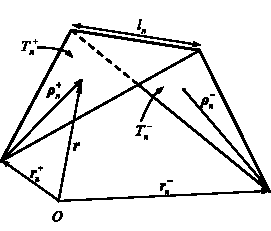
\includegraphics{pica.pdf}
	\caption{RWG 基函数几何参数示意图}
	\label{pica}
\end{figure}
由于时域混合场积分方程是时域电场积分方程与时域磁场积分方程的线性组合,因此时域混合场积分方程时间步进算法的阻抗矩阵特征与时域电场积分方程时间步进算法的阻抗矩阵特征相同。
\begin{equation}
\label{latent_binary_variable}
\mathbf{r}_{i,j}=
\begin{cases}
1,f(\mathbf{x}^{i};\mathbf{w})\cdot f(\mathbf{x}^{j};\mathbf{w})\geq u(\lambda),\\
0,f(\mathbf{x}^{i};\mathbf{w})\cdot f(\mathbf{x}^{j};\mathbf{w})< l(\lambda), 1\leq i,j\leq n.\\
f(\mathbf{x}^{i};\mathbf{w})\cdot f(\mathbf{x}^{j};\mathbf{w}),\text{otherwise},
\end{cases}
\end{equation}

时域积分方程时间步进算法的阻抗元素直接影响算法的后时稳定性,因此阻抗元素的计算是算法的关键之一,采用精度高效的方法计算时域阻抗元素是时域积分方程时间步进算法研究的重点之一。


\subsection{时间基函数}

\subsubsection{时域方法特有的展开函数}

\subsubsection{频域方法特有的展开函数}

\section{入射波}

如图\ref{picb}和图\ref{picc}所示分别给出了参数$E_0=\hat{x}$,$a_n=-\hat{z}$,$f_0=250MHz$,$f_w=50MHz$,$t_w=4.2\sigma$时,调制高斯脉冲的时域与频域归一化波形图。

\begin{figure}[h]
	\subfigure[]{
		\label{picb}
		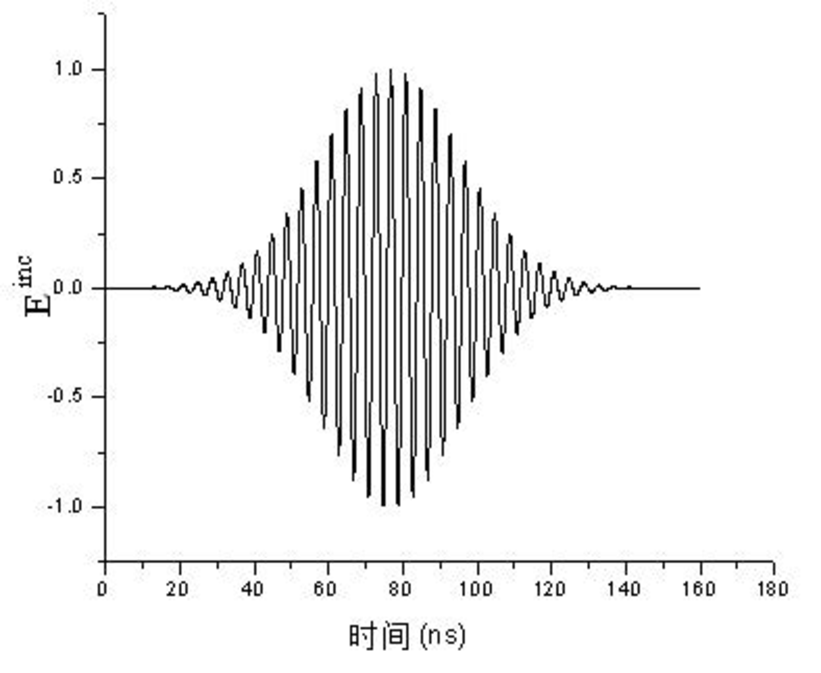
\includegraphics[width=7.3cm]{picb.pdf}}
	\subfigure[]{
		\label{picc}
		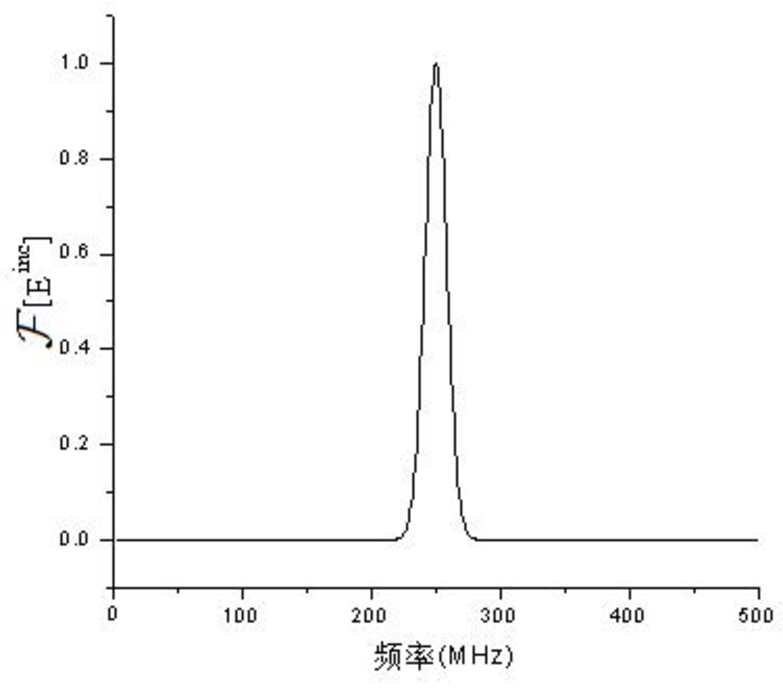
\includegraphics[width=6.41cm]{picc.pdf}}
	\caption{调制高斯脉冲时域与频率波形,时域阻抗元素的存储技术也是时间步进算法并行化的关键技术之一,采用合适的阻抗元素存储方式可以很大的提高并行时间步进算法的计算效率。}
	\label{fig1}
\end{figure}
时域阻抗元素的存储技术\citing{xiao2012yi}也是时间步进算法并行化的关键技术之一,采用合适的阻抗元素存储方式可以很大的提高并行时间步进算法的计算效率。

\section{本章小结}
本章首先从时域麦克斯韦方程组出发推导得到了时域电场、磁场以及混合场积分方程。

\chapter{时域积分方程数值方法研究}
\section{时域积分方程时间步进算法的阻抗元素精确计算}
时域积分方程时间步进算法的阻抗元素直接影响算法的后时稳定性,因此阻抗元素的计算是算法的关键之一,采用精度高效的方法计算时域阻抗元素是时域积分方程时间步进算法研究的重点之一。

\section{时域积分方程时间步进算法阻抗矩阵的存储}
时域阻抗元素的存储技术也是时间步进算法并行化的关键技术之一,采用合适的阻抗元素存储方式可以很大的提高并行时间步进算法的计算效率。

\subsection{时域积分方程时间步进算法产生的阻抗矩阵的特征}
由于时域混合场积分方程是时域电场积分方程与时域磁场积分方程的线性组合,因此时域混合场积分方程时间步进算法的阻抗矩阵特征与时域电场积分方程时间步进算法的阻抗矩阵特征相同。

\subsection{数值算例与分析}

如图3-1(a)所示给出了时间步长选取为0.5ns时采用三种不同存储方式计算的平板中心处 方向的感应电流值与IDFT方法计算结果的比较。如图3-1(b)所示给出了存储方式为基权函数压缩存储方式,时间步长分别取时平板中心处 方向的感应电流计算结果,从图中可以看出不同时间步长的计算结果基本相同。

\begin{algorithm}[H]
	\KwData{this text}
	\KwResult{how to write algorithm with \LaTeX2e }
	initialization\;
	\While{not at end of this document}{
		read current\;
		\eIf{understand}{
			go to next section\;
			current section becomes this one\;
		}{
		go back to the beginning of current section\;
	}
}
\caption{How to wirte an algorithm.}
\end{algorithm}

由于时域混合场积分方程是时域电场积分方程与时域磁场积分方程的线性组合,因此时域混合场积分方程时间步进算法的阻抗矩阵特征与时域电场积分方程时间步进算法的阻抗矩阵特征相同。

\section{时域积分方程时间步进算法矩阵方程的求解}

\section{本章小结}
本章首先研究了时域积分方程时间步进算法的阻抗元素精确计算技术,分别采用DUFFY变换法与卷积积分精度计算法计算时域阻抗元素,通过算例验证了计算方法的高精度。

\chapter{时域积分方程数值方法研究}
\section{时域积分方程时间步进算法的阻抗元素精确计算}
时域积分方程时间步进算法的阻抗元素直接影响算法的后时稳定性,因此阻抗元素的计算是算法的关键之一,采用精度高效的方法计算时域阻抗元素是时域积分方程时间步进算法研究的重点之一。

% \section{时域积分方程时间步进算法阻抗矩阵的存储}
% 时域阻抗元素的存储技术也是时间步进算法并行化的关键技术之一,采用合适的阻抗元素存储方式可以很大的提高并行时间步进算法的计算效率。

\subsection{时域积分方程时间步进算法产生的阻抗矩阵的特征}
由于时域混合场积分方程是时域电场积分方程与时域磁场积分方程的线性组合,因此时域混合场积分方程时间步进算法的阻抗矩阵特征与时域电场积分方程时间步进算法的阻抗矩阵特征相同。

\subsection{数值算例与分析}

如图3-1(a)所示给出了时间步长选取为0.5ns时采用三种不同存储方式计算的平板中心处 方向的感应电流值与IDFT方法计算结果的比较。如图3-1(b)所示给出了存储方式为基权函数压缩存储方式,时间步长分别取时平板中心处 方向的感应电流计算结果,从图中可以看出不同时间步长的计算结果基本相同。

\begin{algorithm}[H]
	\KwData{this text}
	\KwResult{how to write algorithm with \LaTeX2e }
	initialization\;
	\While{not at end of this document}{
		read current\;
		\eIf{understand}{
			go to next section\;
			current section becomes this one\;
		}{
		go back to the beginning of current section\;
	}
}
\caption{How to wirte an algorithm.}
\end{algorithm}

由于时域混合场积分方程是时域电场积分方程与时域磁场积分方程的线性组合,因此时域混合场积分方程时间步进算法的阻抗矩阵特征与时域电场积分方程时间步进算法的阻抗矩阵特征相同。

\section{时域积分方程时间步进算法矩阵方程的求解}

\section{本章小结}
本章首先研究了时域积分方程时间步进算法的阻抗元素精确计算技术,分别采用DUFFY变换法与卷积积分精度计算法计算时域阻抗元素,通过算例验证了计算方法的高精度。


\chapter{时域积分方程数值方法研究}
\section{时域积分方程时间步进算法的阻抗元素精确计算}
时域积分方程时间步进算法的阻抗元素直接影响算法的后时稳定性,因此阻
抗元素的计算是算法的关键之一,采用精度高效的方法计算时域阻抗元素是时域
积分方程时间步进算法研究的重点之一。

\section{时域积分方程时间步进算法阻抗矩阵的存储}
时域阻抗元素的存储技术也是时间步进算法并行化的关键技术之一,采用
合适的阻抗元素存储方式可以很大的提高并行时间步进算法的计算效率。

\subsection{时域积分方程时间步进算法产生的阻抗矩阵的特征}

由于时域混合场积分方程是时域电场积分方程与时域磁场积分方程的线性组
合,因此时域混合场积分方程时间步进算法的阻抗矩阵特征与时域电场积分方程
时间步进算法的阻抗矩阵特征相同。
\subsection{数值算例与分析}
如表\ref{tablea}所示给出了时间步长分别取0.4ns、0.5ns、0.6ns 时的三种存储
方式的存储量大小。

\begin{table}[h]
	\caption{计算$2m\times 2m$理想导体平板时域感应电流采用的三种存储方式的存储量比较。} 
	\begin{tabular}{|c|c|c|c|} 
		\hline  
		时间步长 & 非压缩存储方式 & 完全压缩存储方式 & 基权函数压缩存储方式 \\
		\hline 
		0.4ns & 5.59 MB & 6.78 MB & 6.78 MB\\  
		\hline  
		0.5ns & 10.17 MB & 5.58 MB & 5.58 MB \\  
		\hline  
		0.6ns & 8.38MB & 4.98 MB & 4.98 MB \\  
		\hline  
	\end{tabular}
	\label{tablea}
\end{table}

如图\ref{picd}所示给出了时间步长选取为0.5ns 时采用三种不同存储方式计算的
平板中心处$x$方向的感应电流值与IDFT 方法计算结果的比较,……。如图\ref{pice}
所示给出了存储方式为基权函数压缩存储方式,时间步长分别取0.4ns、0.5ns、0.6ns
时平板中心处$x$方向的感应电流计算结果,从图中可以看出不同时间步长的计算结果基本相同。

由于时域混合场积分方程是时域电场积分方程与时域磁场积分方程的线性组合,因此时域混合场积分方程时间步进算法的阻抗矩阵特征与时域电场积分方程时间步进算法的阻抗矩阵特征相同。

\begin{figure}[h]
	\subfigure[]{
		\label{picd}
		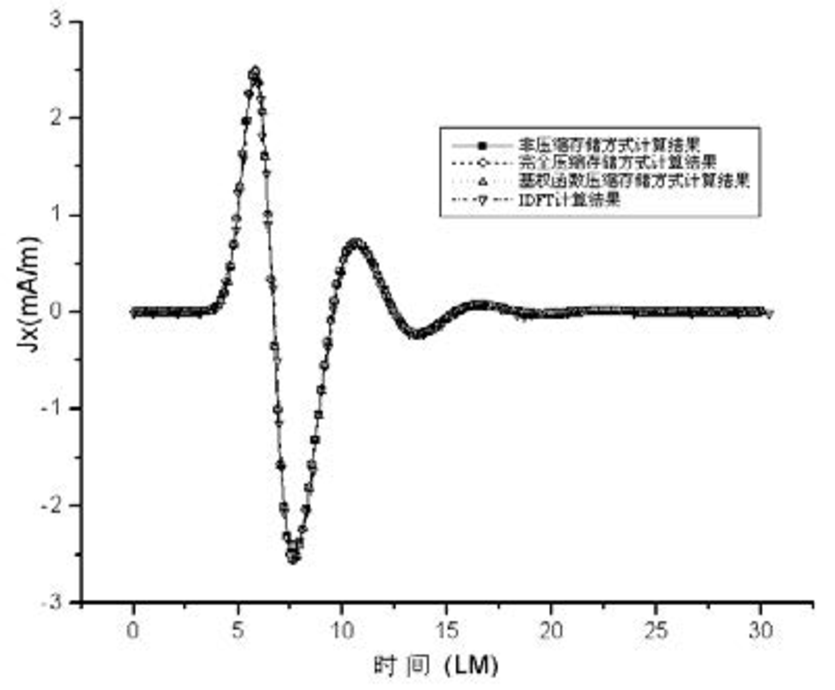
\includegraphics[width=6.77cm]{picd.pdf}}
	\subfigure[]{
		\label{pice}
		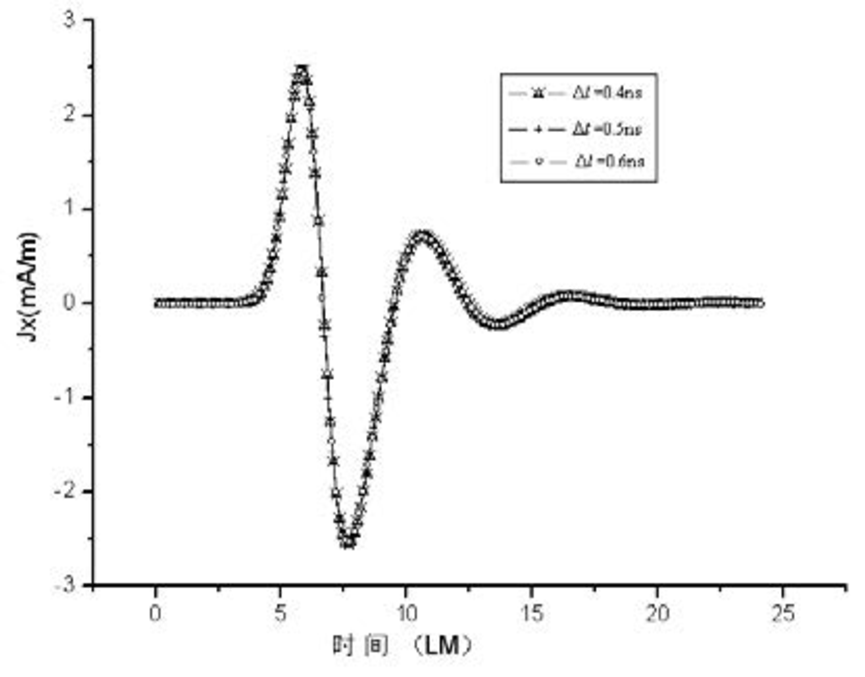
\includegraphics[width=7.04cm]{pice.pdf}}
	\caption{$2m\times 2m$的理想导体平板中心处感应电流$x$分量随时间的变化关系}
	\label{fig2}
\end{figure}


由于时域混合场积分方程是时域电场积分方程与时域磁场积分方程的线性组
合,因此时域混合场积分方程时间步进算法的阻抗矩阵特征与时域电场积分方程
时间步进算法的阻抗矩阵特征相同。
\section{时域积分方程时间步进算法矩阵方程的求解}

\begin{theorem}
	如果时域混合场积分方程是时域电场积分方程与时域磁场积分方程
	的线性组合。
\end{theorem}
\begin{proof}
	由于时域混合场积分方程是时域电场积分方程与时域磁场积分方程的线性组
	合,因此时域混合场积分方程时间步进算法的阻抗矩阵特征与时域电场积分方程
	时间步进算法的阻抗矩阵特征相同。
\end{proof}
\begin{corollary}
	时域积分方程方法的研究近几年发展迅速,在本文研究工作的基础上,仍有以下方向值得进一步研究。
\end{corollary}
\begin{lemma}
	因此时域混合场积分方程时间步进算法的阻抗矩阵特征与时域电场积分方程
	时间步进算法的阻抗矩阵特征相同。
\end{lemma}

\section{本章小结}
本章首先研究了时域积分方程时间步进算法的阻抗元素精确计算技术,分别
采用DUFFY 变换法与卷积积分精度计算法计算时域阻抗元素,通过算例验证了计
算方法的高精度。

\chapter{全文总结与展望}

\section{全文总结}
本文以时域积分方程方法为研究背景,主要对求解时域积分方程的时间步进算法以及两层平面波快速算法进行了研究。

\section{后续工作展望}
时域积分方程方法的研究近几年发展迅速,在本文研究工作的基础上,仍有以下方向值得进一步研究:

%\documentclass{colloqflyer}

%%% Template file for creating CCMS Colloquium Flyers.
%%% $Id: template.tex 285 2009-01-21 21:01:48Z cmc $


%%% The formatting work is all done by the class file, so the
%%% document files just include information that is formatted into
%%% flyer form.

%% Title of the talk.
\title{}

%% Speaker's full name.
\speaker{}

%% Speaker's affiliation (college, company, etc.).
\speakerorg{}

%% Abstract.  Can span multiple paragraphs, just make sure they're
%% all inside the braces.
\abstract{}

%% Date of talk.  As <Day of Week>, <Month> <Day>, <Year>; for
%% example, ``Wednesday, January 21, 2009''.
\date{}

%% Time talk occurs.  Specify time as H:MM~\pm or \am.
\talktime{}

%% Location of talk, in the form <Building> <Room>, <College>.
%% For example, ``Beckman B126, Harvey Mudd College''.
\talklocation{}


%% Refreshment time.  Specify time as H:MM~\pm or \am.
\refreshmenttime{}

%% Refreshment location.  <Building> <Room>, <College>, as with
%% \talklocation.
\refreshmentlocation{}


%% Dinner host.
\host{}

%% You can have a telephone number, an e-mail address, or both.
%% One or the other is required.

%% Dinner host contact telephone.
\hostphone{}

%% Dinner host contact e-mail.
\hostemail{}

%% Colloquium information URL.
\colloqsite{http://ccms.claremont.edu/math-colloquia/}


%%% Now we have the actual document.
\begin{document}

\flyer{}                        % Does all the work.

\end{document}


% misc
% ************************** Thesis Acknowledgements **************************

\begin{acknowledgements}      

For what has been an incredibly rewarding and wonderfully challenging 45 months I have several people to thank, several times over. David, for being a superb supervisor, whose unstinting zen and benevolent wisdom are a template for academic mentorship. Richard and Will, who both played the role of unofficial supervisors and always left their doors ajar. Sharon, whose gravitational pull kept me (and everyone else) in orbit. Dan, Mick and John for providing valuable advice along the way. Steve and Bill who as panel members took a much appreciated interest in my progression. Cam who provided valuable insights into my original project proposal. Various other fantastic UNSW folk that have contributed to the fun, including in no particular order: Sam, Sylvia, Eve, Mitch, Nick, Evan, Jo, Chris, Ben, Anna, Chantel, Francis, David and the Ecostats crew, Angela, Haba, Rhiannnon and the rest of the Big Ecology lab. The brilliant academics of the UCT Botany Dept, and in particular Jeremy and Tony who as honours supervisors made me think differently, in a really good way. My patient parents who have supported me unconditionally in my every pursuit. My generous brother who amongst many other things has done his best to keep me in fashion. My wonderful wife Shan, a mention in the acknowledgements of my thesis almost makes a mockery of your contribution; you rock like Kilimanjaro. Finally, I thank my amazing little Ash Mae, who makes me stop and smell the roses (and the nappies).


\end{acknowledgements}

\thesisloadbibliography[nocite]{reference}

%
% Uncomment following codes to load bibliography database with native
% \bibliography command.
%
% \nocite{*}
% \bibliographystyle{thesis-uestc}
% \bibliography{reference}
%

% comment while no need
%%%%%%%%%%%%%%%%%%%%% appendix.tex %%%%%%%%%%%%%%%%%%%%%%%%%%%%%%%%%
%
% sample appendix
%
% Use this file as a template for your own input.
%
%%%%%%%%%%%%%%%%%%%%%%%% Springer-Verlag %%%%%%%%%%%%%%%%%%%%%%%%%%

\chapter{Chapter Heading}
\label{introA} % Always give a unique label
% use \chaptermark{}
% to alter or adjust the chapter heading in the running head

Use the template \emph{appendix.tex} together with the Springer document class SVMono (monograph-type books) or SVMult (edited books) to style appendix of your book in the Springer layout.


\section{Section Heading}
\label{sec:A1}
% Always give a unique label
% and use \ref{<label>} for cross-references
% and \cite{<label>} for bibliographic references
% use \sectionmark{}
% to alter or adjust the section heading in the running head
Instead of simply listing headings of different levels we recommend to let every heading be followed by at least a short passage of text. Further on please use the \LaTeX\ automatism for all your cross-references and citations.


\subsection{Subsection Heading}
\label{sec:A2}
Instead of simply listing headings of different levels we recommend to let every heading be followed by at least a short passage of text. Further on please use the \LaTeX\ automatism for all your cross-references and citations as has already been described in Sect.~\ref{sec:A1}.

For multiline equations we recommend to use the \verb|eqnarray| environment.
\begin{eqnarray}
\vec{a}\times\vec{b}=\vec{c} \nonumber\\
\vec{a}\times\vec{b}=\vec{c}
\label{eq:A01}
\end{eqnarray}

\subsubsection{Subsubsection Heading}
Instead of simply listing headings of different levels we recommend to let every heading be followed by at least a short passage of text. Further on please use the \LaTeX\ automatism for all your cross-references and citations as has already been described in Sect.~\ref{sec:A2}.

Please note that the first line of text that follows a heading is not indented, whereas the first lines of all subsequent paragraphs are.

% For figures use
%
\begin{figure}[t]
\sidecaption[t]
% Use the relevant command for your figure-insertion program
% to insert the figure file.
% For example, with the graphicx style use
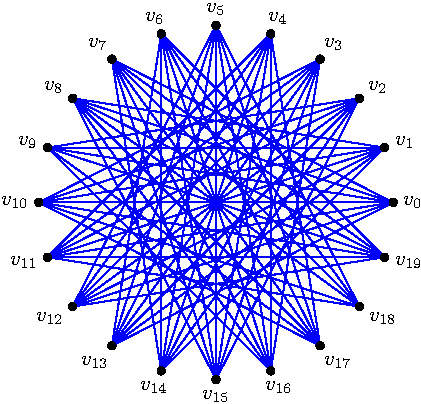
\includegraphics[scale=.65]{figure}
%
% If no graphics program available, insert a blank space i.e. use
%\picplace{5cm}{2cm} % Give the correct figure height and width in cm
%
\caption{Please write your figure caption here}
\label{fig:A1}       % Give a unique label
\end{figure}

% For tables use
%
\begin{table}
\caption{Please write your table caption here}
\label{tab:A1}       % Give a unique label
%
% Follow this input for your own table layout
%
\begin{tabular}{p{2cm}p{2.4cm}p{2cm}p{4.9cm}}
\hline\noalign{\smallskip}
Classes & Subclass & Length & Action Mechanism  \\
\noalign{\smallskip}\hline\noalign{\smallskip}
Translation & mRNA$^a$  & 22 (19--25) & Translation repression, mRNA cleavage\\
Translation & mRNA cleavage & 21 & mRNA cleavage\\
Translation & mRNA  & 21--22 & mRNA cleavage\\
Translation & mRNA  & 24--26 & Histone and DNA Modification\\
\noalign{\smallskip}\hline\noalign{\smallskip}
\end{tabular}
$^a$ Table foot note (with superscript)
\end{table}
%

\thesisloadachievement{publications}

\thesistranslationoriginal
\section{The OFDM Model of Multiple Carrier Waves}



\thesistranslationchinese
\section{基于多载波索引键控的正交频分多路复用系统模型}



\end{document}
